\documentclass[a4paper]{article}
\usepackage[utf8]{inputenc}
\usepackage{indentfirst}
\usepackage[table]{xcolor}
\usepackage{graphicx}

\definecolor{light-gray}{gray}{0.9}

\setlength{\textheight}{690pt}
\setlength{\topmargin}{-0.3in}
\setlength{\headsep}{0pt}
\setlength{\oddsidemargin}{-6mm}
\setlength{\textwidth}{7in}

\title{CS 253: Project Report 2}
\author{Ildar Absalyamov \and Longxiang Chen \and Ali Mohammadkhan}

\begin{document}

\maketitle

\section*{Introduction}

To continue our investigation on functionality of distributed storage systems in presence of network partitions, we have conducted a set of experiments on our candidate storage systems.
These tests are similar in all three candidate storage systems in essence, but due to the specific characteristics of each systems the details could differ. 
For instance, some storage systems have peer-to-peer nature while the others have master-slave architecture, each of these categories needs different test scenarios to be able to carry out comprehensive tests.

In the following sections, we explain our experimental setup and describe various tests, that we have performed. But we would like to point out that these experiments and results are not complete.

\section{Experimental setup description}

Our setup consists of five virtual machines, with Ubuntu Linux installed on all of them along with the considered data storage system. 
These five nodes are connected into a single virtual network, which is located behind a NAT separating it from the host system.
To be able to communicate with the individual nodes of the storage system, we implemented a small client application which was running on a host system, whose requests were routed through the NAT to designated cluster nodes. 
Overall configuration in shown on Figure \ref{fig:cluster}. 

In order to simulate the network partition in this cluster and disconnect nodes N1 and N2 from nodes N3,N4,N5 we configuring iptables firewall on each cluster node to drop packets, received from the partitioned part of the cluster.
Note that the host system is always connected to the cluster nodes, so the partition exists only form the node's point of view.

\begin{figure}[h!]
	\centering
	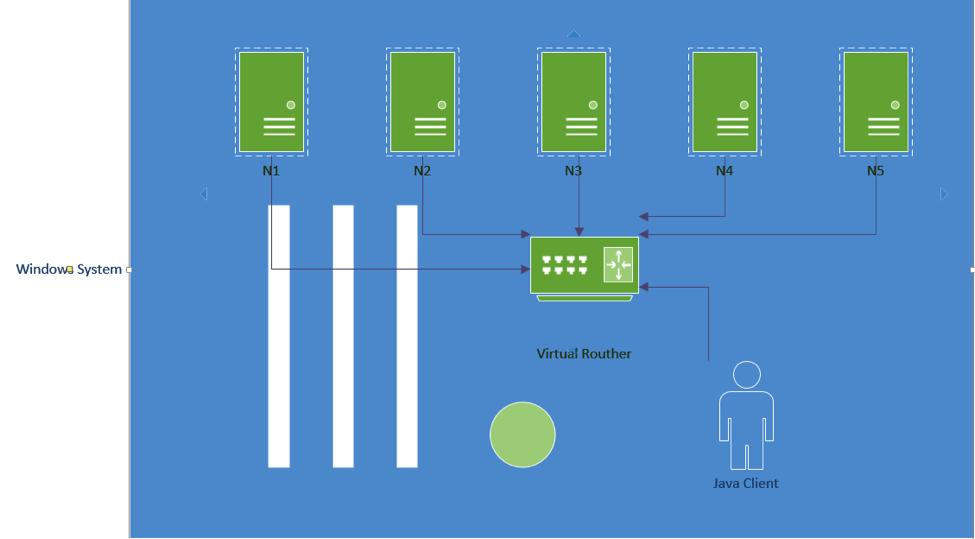
\includegraphics[width=\textwidth]{cluster}
	\caption{Virtual cluster}
	\label{fig:cluster}
\end{figure}

\section{Experiment results}

\subsection{Hazelcast}

For the set of experiments cluster of hazelcast version 3.1 was deployed on the worker nodes. 
We have tested two types of configuration: local cluster and several clusters with WAN replication, each of which was declaring a single distributed map, which was written from the individual worker node.

Tests for the local cluster reveled that out of 2000 writes almost 10\% are lost (result depends on the length of the period, during with the partition was present).
Results show that every record, written on the smaller partition (nodes N1 and N2) is lost, even after partition disappears, which clearly shows the issue with distributed consensus algorithm, used in Hazelcast.
Also it could be noted that when the partition is resolved latency of writes, going to nodes N1 and N2 temporarily increases, which could be explained by the fact that the tuples on these nodes should migrated, when they are rejoining the cluster.

On the other hand configuration, which used WAN replication perfectly survived the network partition, returning all 2000 successfully written tuples.

\subsection{Couchbase}

In our experiments we have used Couchbase 2.1.1 (which is the latest available Community edition version).

Since Couchbase is a peer-to-peer system, there is no need to manually set up master node. Servers obtain their configuration from each other in p2p way.

To start testing and checking the configuration we wrote and read 1000 tuples to Couchbase system and all of them were successful. 
The data is distributed approximately even among different servers (each server has about 200 tuples) and one replication from each tuple is stored on another server. 
Then we turned off one of the servers. It resulted to loosing about 20\% of our writes, in other words, just 803 data tuples were written on Couchbase database and the client was in an attempting loop to write other data tuples to 5th server, which it was never successful, but if we turn the 5th server after writing the data and do the failover over process we can successfully read 1000 written tuples because of provided replication in Couchbase system.

For the network partition tests, all 1000 writes were successful, and then we read the data and all 1000 read were successful too, but as you can see in Figure \ref{fig:partition1} and Figure \ref{fig:partition2}\, the number of replicas are reduced in comparison to prior test, so we designed the next test.

In this test, after writing the 1000 tuples in partitioned mode, we turned off the N5 server and we did the fail over process manually, this time we just were able to read 850 data tuples out of 1000 written tuples in first place. It shows that the replication policy of Couchbase was not successful in presence of network partition. 
Up to now, in Couchbase system, are tests are mostly investigating the availability characteristic, but we will carry out some tests in consistency and performance area before publishing the final report.

\begin{figure}[H]
	\centering
	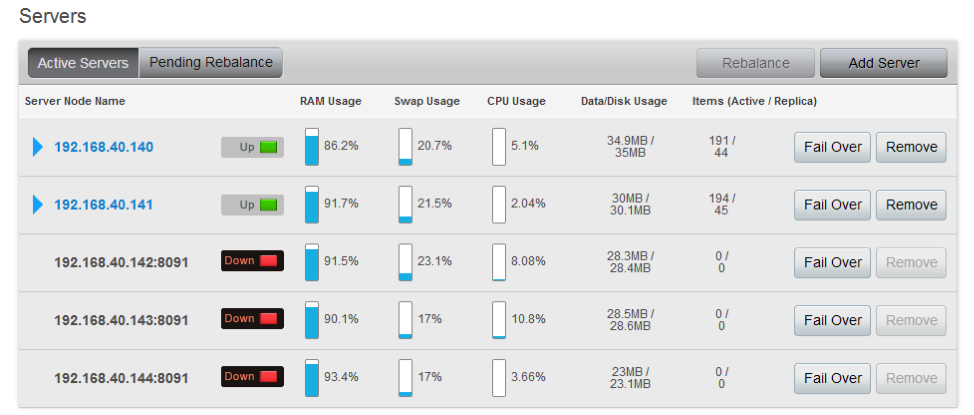
\includegraphics[width=\textwidth]{partition1}
	\caption{1000 tuples writing process form the view of N1-N2}
	\label{fig:partition1}
\end{figure}

\begin{figure}[H]
	\centering
	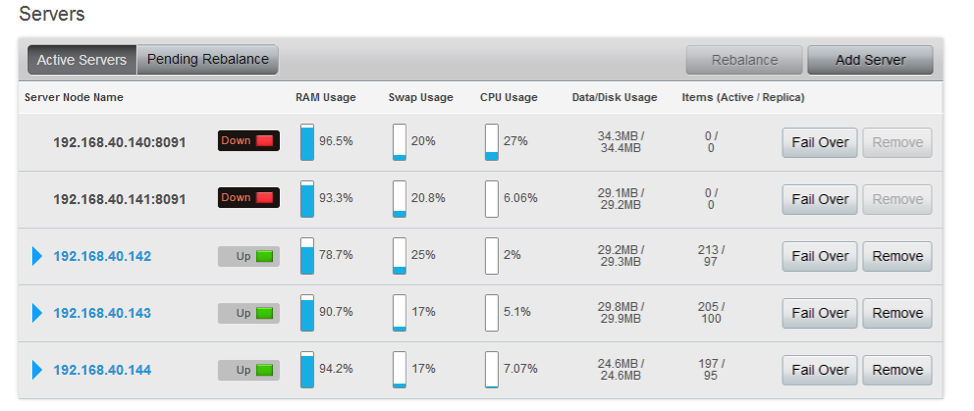
\includegraphics[width=\textwidth]{partition2}
	\caption{1000 tuples writing process form the view of N3-N5}
	\label{fig:partition2}
\end{figure}

\subsection{Voldemort}

In the first report we proposed to use RethinkDB as a third storage system, that we would like to evaluate. But this database is not well documented because it is a new system that few people use it. So it would be hard to configure RethinkDB to support multi-datacenter replca set.

Out backup otion was to use Voldemort distributed key-value storage and configure it for replica set support. We have divided 5 nodes into 2 zones, zone0 has N1, N2 and zone1 has N3, N4 and N5.  However we have encountered some problems with node N1, which was crashing every time we started it.
Possible issues could include mistakes of database configuration, we will try to resolve them as early as possible.

\section*{Contribution}

\begin{table}[hb]
	\centering
	\begin{tabular}{|c|c|}
		\hline
		\rowcolor{light-gray} \textbf{Contributor} & \textbf{Experiments} \\ \hline
		Ildar & Hazelcast  \\ \hline
		Lonxiang & Voldemort  \\ \hline
		Ali & Couchbase  \\ \hline
	\end{tabular}
\end{table}

\end{document}